% Results section for "Multi-Fidelity Training Reshapes Uncertainty Decomposition
% in Atomistic Models".
%
% Figure paths assume the PDFs in new_figures/out/ are reachable as out/*.pdf.
% When this file is moved into the manuscript tree, either copy out/*.pdf next to
% it or add \graphicspath{{new_figures/out/}} to the preamble.
%
% Every number quoted below is the mean over the five dataset splits with a
% two-sided 95% Student-t interval (df = 4), recomputed from the per-configuration
% caches by the scripts in new_figures/.

\section{Results}
\label{sec:results}

We analyse uncertainty along two axes that the literature often conflates: whether
uncertainty \emph{ranks} configurations by error (AUSE, Spearman) and whether its
\emph{magnitude} matches the observed error (ENCE). Section~\ref{sec:results:final}
studies the converged models (RQ1), Section~\ref{sec:results:shift} contrasts the two
distribution shifts and post-hoc recalibration (RQ3), Section~\ref{sec:results:dynamics}
follows the whole optimisation trajectory (RQ2), and Section~\ref{sec:results:al}
tests whether the resulting uncertainty is useful for data acquisition.

\paragraph{Evaluation protocol.}
Every metric is computed within a dataset split from a 10-member ensemble, and then
summarised over the five splits as a mean with a two-sided 95\% Student-t interval
(df${}={}$4); strictly positive quantities shown on logarithmic axes use geometric
means with log-space intervals. Splits, not ensemble members, are the unit of
replication. Test configurations whose smallest interatomic distance falls below the
smallest one occurring anywhere in that split's own training data are excluded, for
every protocol and every uncertainty signal alike. This training-support filter reads
geometry only, so it cannot select on the quantity being evaluated; it removes 13--16
of 5000 Energy-OOD configurations per split and essentially nothing elsewhere. Those
configurations are compressed far below the repulsive wall covered by training, where
a single configuration can dominate a mean of squares; we therefore report them as
outside the domain of validity rather than as evidence about uncertainty. LF-only
models are scored against DFT labels and are shown only where that comparison is
meaningful.

\subsection{Pretraining improves ranking, but not calibration}
\label{sec:results:final}

\begin{figure}[t]
  \centering
  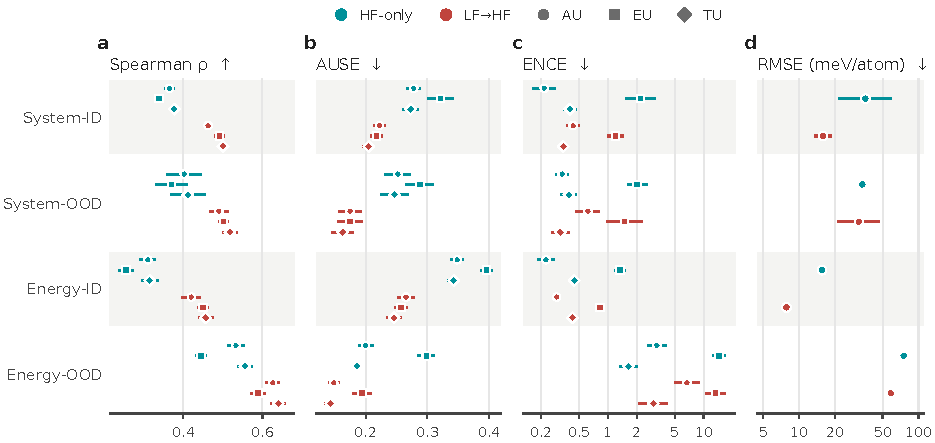
\includegraphics[width=\linewidth]{out/fig2_final_summary.pdf}
  \caption{\textbf{Converged models: multi-fidelity training improves error ranking on
  every test set, while calibration does not follow.} Each row block is a test set and
  each column a metric; colour denotes the training protocol (teal HF-only, red
  LF$\rightarrow$HF) and marker shape the uncertainty signal (circle AU, square EU,
  diamond TU). Markers are means over five dataset splits, bars are 95\% Student-t
  intervals; ENCE and RMSE use logarithmic axes with geometric means. LF$\rightarrow$HF
  attains higher Spearman and lower AUSE for all three signals on all four test sets,
  and lower RMSE everywhere except System-OOD, where the two protocols tie. AU is
  nevertheless better calibrated for HF-only on all four test sets, and the wide
  HF-only System-ID RMSE interval is caused by a single split-0 configuration inside
  the training support with an error of $-4.4$~eV/atom.}
  \label{fig:final}
\end{figure}

Figure~\ref{fig:final} summarises the converged models. Low-fidelity pretraining
improves the \emph{ranking} quality of uncertainty on every test set and for every
signal. For total uncertainty, Spearman rises from $0.377\pm0.012$ to
$0.500\pm0.009$ on System-ID, from $0.411\pm0.044$ to $0.518\pm0.019$ on System-OOD,
from $0.315\pm0.022$ to $0.457\pm0.019$ on Energy-ID and from $0.556\pm0.018$ to
$0.640\pm0.019$ on Energy-OOD; TU AUSE falls correspondingly ($0.273\to0.205$,
$0.247\to0.163$, $0.343\to0.246$ and $0.186\to0.143$). Accuracy improves as well, by
roughly a factor of two in domain ($15.60\pm0.35$ to $7.86\pm0.34$~meV/atom on
Energy-ID) and by $22\%$ on Energy-OOD ($75.3\pm5.5$ to $58.7\pm5.0$~meV/atom), with
the single exception of System-OOD, where the protocols are indistinguishable
($33.97\pm3.04$ vs.\ $32.95\pm11.22$~meV/atom).

Calibration behaves differently. Aleatoric uncertainty is \emph{better} calibrated
without pretraining on all four test sets (ENCE $0.220$ vs.\ $0.436$ on System-ID,
$0.335$ vs.\ $0.632$ on System-OOD, $0.228$ vs.\ $0.292$ on Energy-ID and $3.30$
vs.\ $6.86$ on Energy-OOD), and under energy extrapolation the same reversal reaches
total uncertainty ($1.66\pm0.37$ for HF-only vs.\ $3.07\pm1.15$ for
LF$\rightarrow$HF). Epistemic uncertainty is the worst-calibrated signal throughout
(ENCE between $0.8$ and $14.6$) yet, after pretraining, ranks almost as well as TU.
Multi-fidelity training therefore buys a better ordering of errors and a lower error,
but it does not buy uncertainties of the right size: the two properties must be
reported separately.

\subsection{The type of shift decides whether ranking and calibration agree}
\label{sec:results:shift}

\begin{figure}[t]
  \centering
  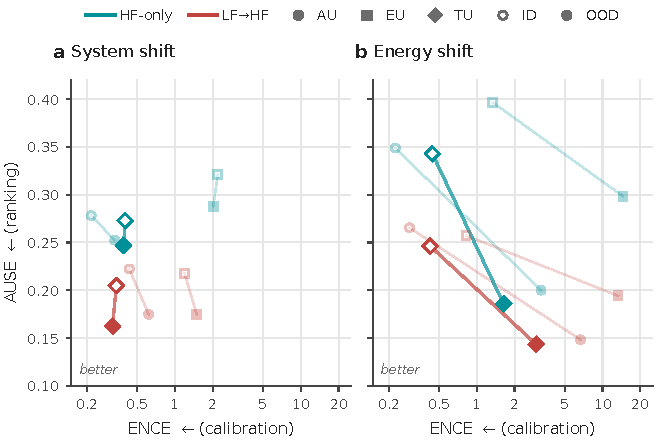
\includegraphics[width=\linewidth]{out/fig4_rank_vs_calibration.pdf}
  \caption{\textbf{Ranking and calibration decouple under energy extrapolation, and
  post-hoc recalibration does not transfer.} \textbf{(a)} Calibration (ENCE, $x$) against
  ranking (AUSE, $y$); the lower-left corner is best. Arrows join the in-domain to the
  shifted test set for total uncertainty, one arrow per protocol; AU and EU are the
  hollow markers. System shift moves the models little, whereas energy shift moves them
  \emph{left-and-up}: ranking improves while calibration degrades by a factor of
  $3.7$--$7.2$. \textbf{(b)} Effect of isotonic recalibration fitted on the validation
  set: hollow markers before, filled after, one row per protocol and signal. Under system
  shift recalibration repairs EU (HF-only $2.05\to0.48$); under energy shift it makes AU
  and TU substantially worse for both protocols.}
  \label{fig:shift}
\end{figure}

Figure~\ref{fig:shift}a places both test regimes in the ENCE--AUSE plane. Moving from
System-ID to System-OOD barely changes either coordinate (TU: AUSE $0.273\to0.247$ and
ENCE $0.404\to0.394$ for HF-only; $0.205\to0.163$ and $0.343\to0.324$ for
LF$\rightarrow$HF). Moving from Energy-ID to Energy-OOD instead \emph{improves} ranking
markedly (TU AUSE $0.343\to0.186$ and $0.246\to0.143$) while degrading calibration by
$3.7\times$ and $7.2\times$ (TU ENCE $0.445\to1.657$ and $0.427\to3.072$). Under energy
extrapolation the models still know \emph{which} configurations they will get wrong, but
systematically underestimate \emph{by how much}; a held-out ranking metric alone would
declare these models more reliable out of domain than in it.

This asymmetry survives recalibration (Figure~\ref{fig:shift}b). An isotonic map fitted
on in-domain validation data repairs the badly scaled epistemic signal under system shift
($2.05\to0.48$ for HF-only, $1.56\to0.38$ for LF$\rightarrow$HF), leaving TU unchanged for
HF-only ($0.39\to0.36$) but degrading it for LF$\rightarrow$HF ($0.32\to0.52$); under
energy extrapolation the same procedure inflates the calibration
error of AU and TU for both protocols (TU $1.66\to6.71$ for HF-only and $3.07\to8.26$ for
LF$\rightarrow$HF). Recalibration learned where the model interpolates is therefore not
merely insufficient but actively harmful where it extrapolates.

\subsection{Training dynamics: the high-fidelity stage is what breaks AU}
\label{sec:results:dynamics}

\begin{figure}[t]
  \centering
  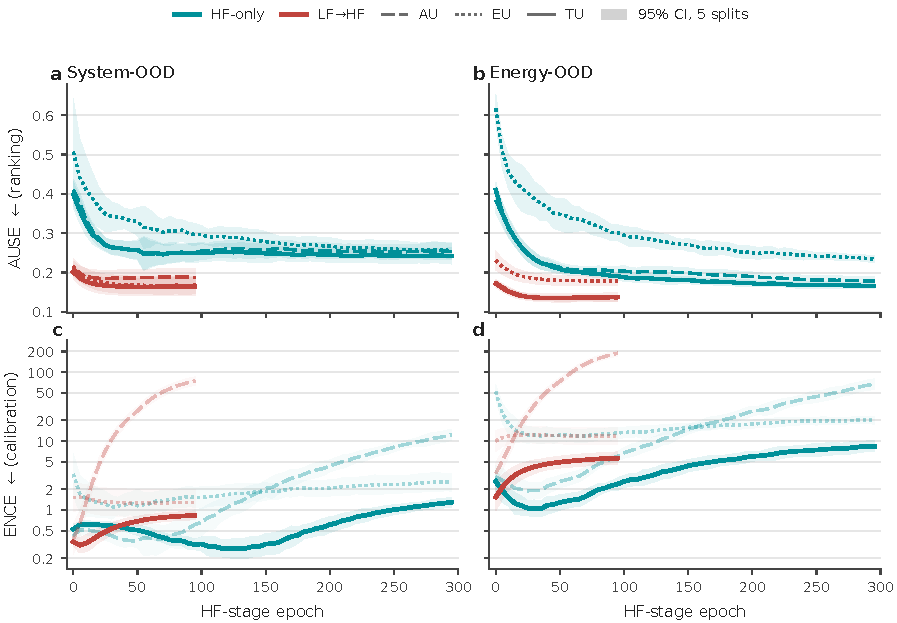
\includegraphics[width=\linewidth]{out/fig3_hf_dynamics.pdf}
  \caption{\textbf{The high-fidelity stage starts from a better uncertainty when it is
  preceded by low-fidelity pretraining, and never loses that advantage.} Total-uncertainty
  ranking (top) and calibration (bottom) on the OOD test sets against the epoch of the
  high-fidelity stage, for HF-only training from scratch (teal, 300 epochs) and the CC
  fine-tuning stage of LF$\rightarrow$HF (red, 100 epochs). Faint lines are the five-split
  mean per evaluated epoch, bold lines its exponential moving average, bands the 95\%
  interval. After a single fine-tuning epoch LF$\rightarrow$HF already ranks better
  (TU AUSE $0.201$ and $0.172$) than HF-only does after 300 epochs ($0.242$ and $0.165$).
  Calibration degrades monotonically during the high-fidelity stage in both protocols.}
  \label{fig:hfdynamics}
\end{figure}

\begin{figure}[t]
  \centering
  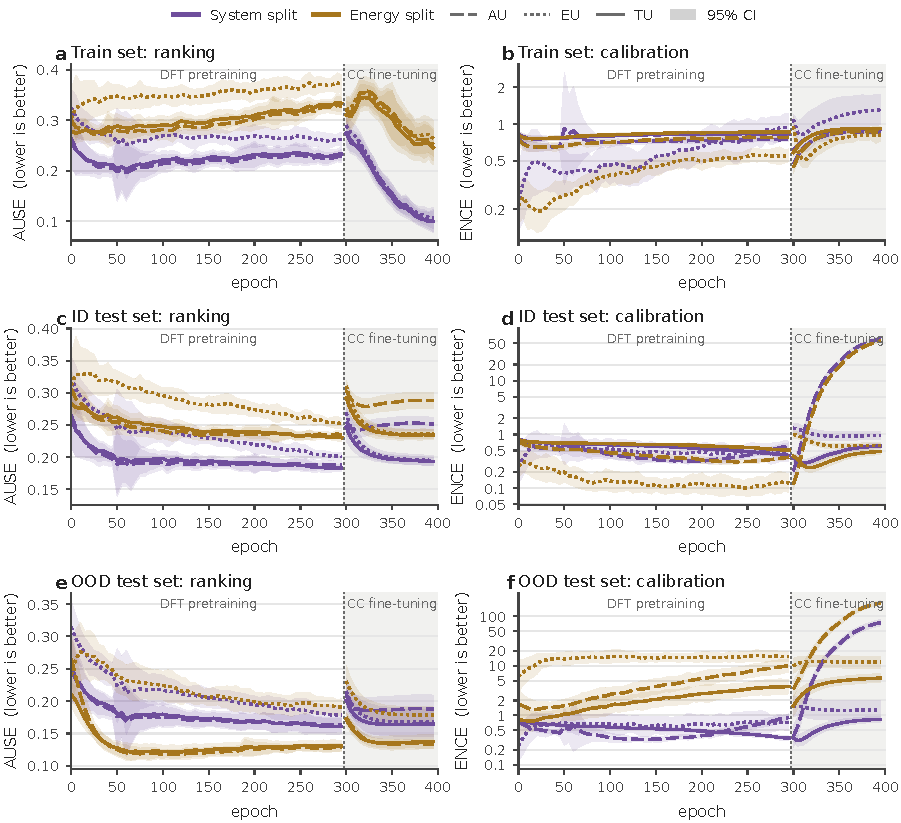
\includegraphics[width=\linewidth]{out/fig5_decomposition.pdf}
  \caption{\textbf{Fine-tuning makes AU overconfident on unseen data while EU keeps total
  uncertainty usable; the decomposition does not reorganise with depth into the energy
  tail.} \textbf{(a)--(g)} follow LF$\rightarrow$HF through DFT pretraining (epochs
  0--299) and CC fine-tuning (300--399, shaded), on its own training data (a,b), the ID
  test set (c,d) and the OOD test set (e,f); colour is the split (purple system, brown
  energy) and line style the signal (dashed AU, dotted EU, solid TU), with 95\% bands.
  \textbf{(g)} mean EU over mean AU on the OOD test set. \textbf{(h)} converged models on
  the energy split: median per-configuration EU/AU in Energy-ID and in within-system
  energy-quantile bins of Energy-OOD. Fine-tuning drives AU ENCE from $0.99$ to $81.9$
  (System-OOD) and from $10.9$ to $207$ (Energy-OOD), while TU stays two orders of
  magnitude lower; on the training data itself ranking keeps improving (TU AUSE
  $0.236\to0.098$), so the failure is specific to unseen data. The median EU/AU ratio
  never exceeds one in any bin.}
  \label{fig:decomposition}
\end{figure}

Figure~\ref{fig:hfdynamics} isolates the high-fidelity stage. Pretraining does not merely
accelerate convergence: at the very first CC epoch the pretrained ensemble already ranks
errors better (TU AUSE $0.201$ on System-OOD and $0.172$ on Energy-OOD) than a model
trained from scratch on CC reaches after 300 epochs ($0.242$ and $0.165$), and the gap
never closes. Calibration moves the other way for both protocols: TU ENCE grows from
$0.53$ to $1.36$ (HF-only) and from $0.35$ to $0.83$ (LF$\rightarrow$HF) on System-OOD,
and from $2.59$ to $8.43$ and $1.54$ to $5.72$ on Energy-OOD. The high-fidelity stage is
thus where uncertainty magnitudes deteriorate, irrespective of how the stage was
initialised.

Figure~\ref{fig:decomposition} follows the full multi-fidelity trajectory and identifies
which component fails. During DFT pretraining, OOD ranking improves steadily (TU AUSE
$0.249\to0.161$ on System-OOD, $0.210\to0.131$ on Energy-OOD) and all three signals stay
close to calibrated (TU ENCE $0.335$ and $3.96$ at the end of pretraining). Fine-tuning
then breaks the aleatoric head on unseen data: AU ENCE rises from $0.99$ to $81.9$ on
System-OOD and from $10.9$ to $207$ on Energy-OOD, with the same effect on the ID test
sets ($0.69\to67.2$ and $0.40\to60.5$). Total uncertainty degrades far less
($0.34\to0.83$ and $3.96\to5.72$) because the epistemic term partly absorbs the
deficit. The failure is specific to data the model has not fitted: on its own CC training
data, ranking improves throughout fine-tuning (TU AUSE $0.236\to0.098$ on the system
split) and TU ENCE stays near one ($0.83\to0.90$). A small ensemble-based epistemic term
is therefore not a refinement of the mean-variance head but the component that keeps the
predictive variance usable after fine-tuning.

Finally, Figure~\ref{fig:decomposition}h tests the common expectation that epistemic
uncertainty takes over as configurations move deeper into the energy tail. With a robust
per-configuration estimator, the median EU/AU ratio stays below one in every bin and for
every protocol: it rises only mildly from in-domain to mid-tail (LF$\rightarrow$HF
$0.59\to0.91$, HF-only $0.39\to0.58$) and falls again in the highest-energy bin
($0.72$ and $0.51$). Multi-fidelity training does shift the balance towards EU relative
to both single-fidelity baselines, but the decomposition does not invert with depth into
the tail; mean-based summaries that suggest otherwise are dominated by a handful of
configurations outside the training support.

\subsection{Consequence for data acquisition}
\label{sec:results:al}

\begin{figure}[t]
  \centering
  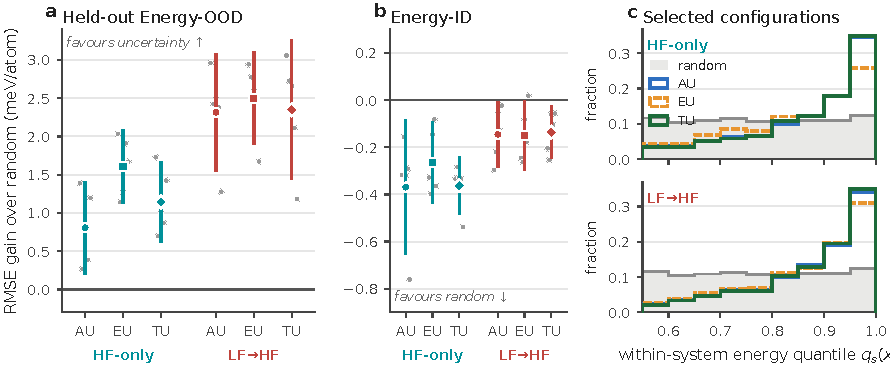
\includegraphics[width=\linewidth]{out/fig6_acquisition.pdf}
  \caption{\textbf{Uncertainty-guided acquisition beats random selection, and the
  advantage is larger after low-fidelity pretraining.} A single acquisition round selects
  500 of 2500 pool configurations and is evaluated on the disjoint held-out half of
  Energy-OOD. \textbf{(a)} RMSE reduction relative to random selection (positive favours
  uncertainty-guided acquisition); markers are five-split means with 95\% intervals, grey
  dots the individual splits. \textbf{(b)} the same on the in-domain test set, where all
  strategies pay a small cost. \textbf{(c)} within-system energy quantile $q_s(x)$ of the
  selected configurations; the grey histogram is random selection, which reproduces the
  pool. Every signal and protocol improves on random out of domain, by $1.6$--$2.9\times$
  more after pretraining; the selected batches concentrate on the top decile of each
  molecule's energy range (median $q_s\approx0.91$ vs.\ $0.78$ for the pool).}
  \label{fig:acquisition}
\end{figure}

If the ranking advantage of Section~\ref{sec:results:final} is real, it should be
exploitable. We split the Energy-OOD set into a 2500-configuration acquisition pool with
hidden labels and a disjoint 2500-configuration test set, reveal 500 labels chosen by each
signal, and continue training each of the ten members
(Figure~\ref{fig:acquisition}). All six combinations of protocol and signal beat random
selection on the held-out OOD test, with intervals excluding zero: after pretraining the
gains are $2.32\pm0.77$ (AU), $2.50\pm0.61$ (EU) and $2.35\pm0.91$~meV/atom (TU) against a
random-selection baseline of $53.1$~meV/atom, whereas without pretraining they are
$0.81\pm0.61$, $1.60\pm0.49$ and $1.14\pm0.53$~meV/atom against a baseline of
$67.4$~meV/atom. Pretraining thus multiplies the benefit of uncertainty-guided acquisition
by $1.6$--$2.9\times$, and it also levels the three signals: after pretraining their gains
are within $0.2$~meV/atom of each other, whereas without pretraining EU gives the largest
gain and AU the smallest, consistent with AU being the component that fine-tuning
miscalibrates. With five splits these within-protocol differences are not individually
resolved. The cost in
domain is small and comparable across strategies ($-0.14$ to $-0.37$~meV/atom).
Figure~\ref{fig:acquisition}c shows what the signals actually select: every uncertainty
strategy concentrates on the high-energy end of each molecule's range (median
$q_s = 0.88$--$0.91$ against $0.78$ for the pool), with HF-only EU reaching least deep.
Uncertainty estimated after multi-fidelity training is therefore not only better ordered
in an offline metric, it also selects better training data.
